%
% $Id: ch02_relatedwork
%
%   *******************************************************************
%   * SEE THE MAIN FILE "AllegThesis.tex" FOR MORE INFORMATION.       *
%   *******************************************************************
\chapter{Related Work}\label{ch:relatedwork}

\section{Secondary Sources}

\subsection{SCATS}
The Sydney Coordinated Adaptive Traffic System (SCATS) is one of the most commonly used traffic monitoring and regulating systems used today and has been deployed in 154 cities across 25 different countries, though under different names.  It was developed in late 1979 by A.G. Sims and K. W. Dobinson and was used primarily on major arteries in urban environments.  It is a dynamic on-line and real-time system which manages the timing of signal phases of different intersections to find the best fitting solution for the current traffic situation.  It also allows and incorporates real-time pedestrian traffic flows, public vehicle transportation, as well as public vehicle priority systems.  The priority system is generally associated with the tram and bus system where there are  high, medium, and low priority levels, with  low priority vehicles waiting their turn, while high priority vehicles skip all other phases to get to their call locations.  The system supports three levels of control as well, a local level, a master level, and the control center.  The control center is the central computer hub, which supplies all area-based traffic control and urban based traffic control(UTC) with information it keeps in its logs, and allows the entire system to be monitored from a central location with a holistic view of the system.  The master level is one level below that and is in charge of regional areas; it has a small amount of local storage for data as well as a control system and a logging system.  Finally, the lowest level of control is given to the local controller, which consists of a road side box at each intersection. These boxes contain the hardware to control the nearby intersections and allow for emergency updates as well as immediate control over particular intersections.  All of these different sections of the system are in constant communication with each other through the telephone lines, resulting in a robustly dynamic system\cite{SCATS}.

The drawback to this system is that it requires the purchase and installation of a large amount of hardware for the system to be implemented.  Back in 1980, when the paper was written, the cost of installing a system, not including the additional costs associated with rerouting traffic, etc., averaged 2.5 million dollars.  Additionally this system has an associated monthly cost for the use of the telephone wires, which the researchers estimated would be about  220 thousand dollars a year.  Further,  this system cannot be implemented immediately due to the fact that the city must take the time to install it\cite{SCATS}. 

This system boasts a 20 percent reduction in accidents and 20-48 percent reduction in delays, leading to an estimated 10 million dollars in fuel savings, and an 18 percent reduction in carbon monoxide(CO) emissions.  One of the final benefits that these researchers saw in their implementation was related to directing the preferred traffic flow of commuters.  They argued that by reducing delays and traffic congestion on the main arteries of routes into and out of popular areas, commuters were more likely to take the intended routes.  This in turn caused a reduction of impatient commuters attempting to cut through neighborhood areas in order to escape the delays associated with the main routes \cite{SCATS}.
	
\subsection{Vehicle-to-Vehicle}
Another recent topic of research in the field is the change from physical control devices to virtual, in-car devices, relying entirely upon the surrounding vehicles to gather data about the state of the intersection and to make timing decisions.  Research was presented in 2010 by Ferreira, et al.\cite{V2V} as a solution to overcome several problems which other traffic control systems have, such as the SCATS traffic system.  The researchers cite that the motivation behind this study lies within the problems that traditional traffic methods have, and introduce through its simplicity of sensor systems.  They say that the sensors in these physical systems, allow the controlling computers to make intelligent decisions based on their observations, however introduce the problem naivete of the rest of the environment, which can lead to possible large miscalculations of the actual state of the intersection.  For example, if the sensors which decide the length of the queue are only 200 feet back from the light, if a car is on that sensor, there is a chance that the queue goes beyond that distance and extends for a significant distance\cite{V2V}.  

To remedy this, the authors propose a traffic control system that is completely encapsulated within the car, from data collection, to decision making, and control signal indication, acting as a completely self-organized system.  Ferreira et al. make the assumptions that firstly, all of the vehicles in the system are equipped with a dedicated short range communication (DSRC) device, tuned to a specific channel so that the cars will be able to find each other, the cars are equipped with an up to date roadmap and accurate global positioning system (GPS), and some sort of dedicated Application Unit (AU).  The step process that this system proposes to implement involves firstly, establishing a Virtual Traffic Light (VTL) protocol with all the surrounding cars approaching the intersection to indicate that a traffic signal will be used at the upcoming intersection.  Following this step, the vehicles approaching the intersection are responsible for electing a leader node, which will be responsible for creating the VTL and broadcast the traffic light message to all surrounding node, as well as be responsible to serve as the primary form of infrastructure for that instance of the intersection.  This leader is elected using a predetermined algorithm so that there is no conflict; however, two rules apply to this leader node.  First, it must be stopped at the intersection and remain there while it is leading that intersection, and second, it must be the closest to the center, or front, of the queue in its lane.  This second criteria is strictly there to optimize communication.  Following this, the leader will broadcast the lighting signals to all nearby vehicles on an individual basis, which is why an accurate GPS is required in order to ensure that vehicles are correctly interpreted as to lane location.  The researchers conducted several simulations based on the major city of Porto, Portugal, and concluded that there was a significant benefit and case for viability\cite{V2V}.  While this system is a fascinating one, the researchers also made it clear that this system should primarily be used where traffic lights are not necessarily required, and that it should supplement the existing system.  Additionally, this research presumed that all of the vehicles in the environment are outfitted with specific hardware to allow this sort of communication to work.  Even if this were to be the protocol for a country, there are still several issues that could arise.  For example, if some country in Europe were to adopt this system and implement it completely as a substitute for the physical system, if any other vehicle from some outside country were to come into the nation, there is a chance that their car may not have the hardware to support it.  This could result in car accidents and other forms of delay for the entire system.

\subsection{Vehicle-to-Infrastructure}
In the case that a city does not wish to completely replace its existing system, there are cases where the idea of a real-time, intelligent system which uses information it gathers from nearby vehicles, instead of the environment like the SCATS case, to allow a traffic controller to make enlightened decisions about the signal selections.  Vehicular Ad-Hoc Network (VANET) is a very commonly explored technology which is used to collect and interpret information about nearby cars' speeds and positions.  Avzekar and Moon, 2014\cite{V2I}, propose a system which will use this VANET technology to interpret and gather information about the density of traffic approaching an intersection, and to make intelligent decisions about regulating this traffic; while favoring emergency vehicles, allowing them to run lights or giving them direct routes to their destinations.  The premise of this system is encapsulated in \ref{Figure 1}, which illustrates exactly how the system will work.  Note that in the diagram below, the RF receiver stands for a radio frequency receiver.
\begin{figure}[h]
	\centering	
	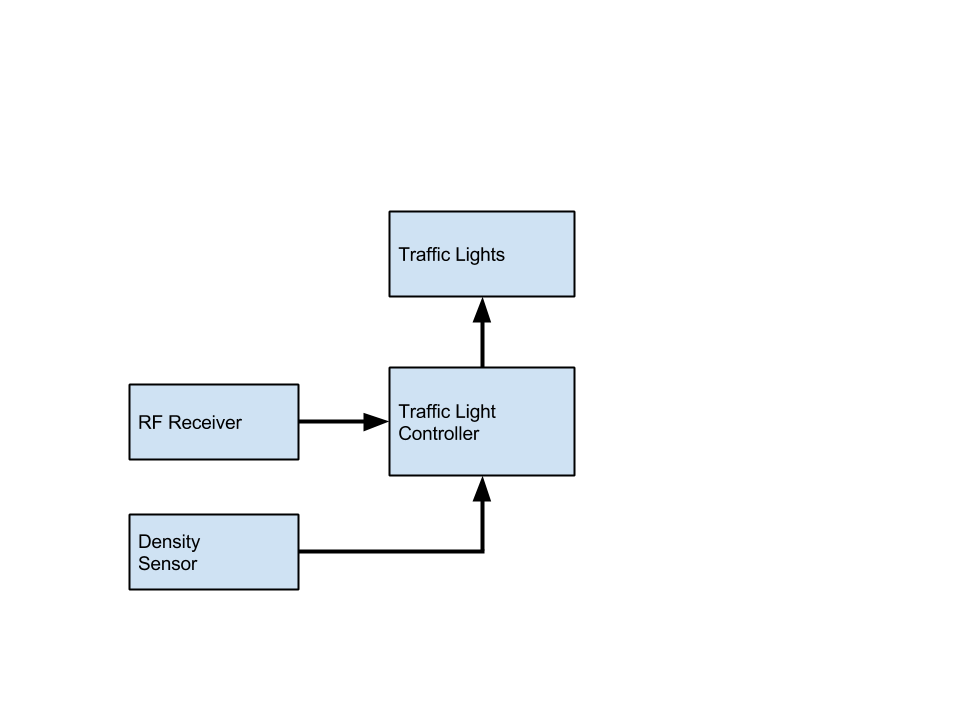
\includegraphics[scale=.4]{images/vanet.png}
	\caption{Block diagram of adaptive traffic system equipped with VANET}
	\label{Figure 1}
\end{figure}
The first methodology proposed by these researchers deals with optimizing traffic light timing based on the volume and density of the incoming traffic.  Using VANET, they make the case that they will be able to manage the system and to allocate greater time to higher flow streets at an intersection and significantly less time to lower density streets.  This is logical and generally the goal of any optimization of traffic control system.  The second goal of their implementation is one of greater interest, however, and deals with the priority system for emergency vehicles.  They propose that a city's emergency vehicles be outfitted with radio frequency transmitters to communicate with the traffic light controller as needed.  In this situation, all other nearby lights besides those in the emergency vehicle's lane will be immediately turned red until that ambulance, fire truck, or police car passes, after which the lights will resume their regular operation.  Using simulations, Avzekar and Moon were able to see that this approach to solving the traffic problem had no negative effects and resulted in consistent, smooth traffic flow.  However, by failing to make a cost-benefit of the VANET system, they render their research slightly inconclusive\cite{V2I}.  There are problems with this system that are not make mention, yet are definitely present.  First, VANET once again requires that \textit{all} vehicles in a system have certain pieces of hardware installed in order for the system to work.  Second, since security measures were not addressed, there is a chance that the radio frequency waves could be vulnerable to attacks. 

\subsection{Reinforced-Learning}
Although the previous examples of traffic optimization covered methods which used sensors and real time techniques in order to adequately manage systems, there are several ways in which a traffic system can be optimized through the use of algorithms.  One paper that showed promising signs of ways to optimize this system used collaborative reinforced-learning techniques in order to support many of the unpredictable aspects associated with urban UTC.  Salkham et al., 2008, propose using a collaborative reinforced learning system for the optimization process for several reasons, the most important being that reinforced learning is a great approach in unstable conditions where the flux of these systems are inevitable.  Further, using the collaborative method over the traditional method allows for the implementation to affect the decentralized aspect of traffic optimization. Through a comparative study, they were able to show that both the traditionally reinforced learning technique and the collaborative reinforced learning technique reduce average wait time per arrived vehicle; however, they noticed that the collaborative technique was able to improve the overall quality of the optimization.  Unfortunately, this study was done on a microscopic scale with regard to the simulation and detailed vehicles' behavior in a real city.  The microscopic aspect of the simulator signifies that it tracks vehicles moving around the network on a second or sub-second basis, making it very accurate after the initial ``warm-up" period.  Thus the study's are very promising and might, in fact, translate well to real world application\cite{CRL}.  


\section{Primary Sources}

Ceylan and Bell, 2004\cite{biGA}, cover two problems in one study: area traffic control optimization and user routing.  They present the problem as an equilibrium network design problem rather than as a scheduling problem.  Additionally, they call a known simulator named TRANSYT-7F to help evaluate the light timings of their genetically modified system.  The network used for this simulation is small having only six control junctures, or intersections.  Still, their findings are promising, suggesting that a genetic optimization can solve this type of problem.  They arrive at three major conclusions: first, that this process shows an improvement of around 34 percent by the 75th generation; second, that the solution is strongly affected by the initial set of timings; and third, that depending on the model, there can be a huge disparity in total optimization time, from 16.5 seconds to 18.4 hours\cite{biGA}.  The implication of these conclusions for the research project at hand is that flow patterns can be repeated multiple times with different initial traffic timings.  The traffic flow pattern the utilized were static, and tests were run multiple times with random starting traffic timing patterns determined by an algorithm.  This provided sufficient results to determine whether an optimization process failure was due to the traffic flow set-up, or by the initial starting values of that optimization run. 

Another example in which GAs not only worked but outperformed other stochastic algorithms is documented by Yun and Park, 2006\cite{CORISM}, in a paper on the application of optimization methods applied to an urban corridor.  They survey two existing optimization models for traffic timing, SYNCHRO(Husch and Albeck 2004) and CORISM.  CORISM is the most recent addition to the TRANSYT-7F model, which uses a microscopic model and includes three different heuristics: a GA, simulated annealing, and an optimization engine called OptQuest.   In their conclusion, the authors highlight that the recently introduced GA aspect of CORISM outperformed every other optimization method to which it was compared.  These include the other heuristics of CORISM, as well as the commonly used SYNCHRO.  While discussing future works, they caution future researchers that the performance of GAs is closely correlated to the original parameter settings.  Further, they warn that running these optimizations can be time intensive.  By showing that the GA outperformed the other heuristics by a rather large margin, around 15.2 percent in their measures of effectiveness, they influenced this researcher to focus on the implementations of a genetic algorithm rather than some other method\cite{CORISM}.

While the time and scope of this research paper do not permit the use of a multi-objective GA, there have been occasions where this method has been applied to traffic control configuration problems with some success.  One such example, completed by Li, Tao, and Chen, 2013\cite{moGA}, focuses on implementing a multi-objective GA on an oversaturated intersection.  The environment scale varied between one- and two-intersection environments.  Their study was motivated by the observation that many modern traffic control systems lack the ability to efficiently deal with circumstances where the amount of congestion overflows the normal boundaries.  The variables they identify include queue length, delay, cycle length, and others.  They determine that the number of variables, deems a multi-objective GA called NSGA-II to be the most appropriate approach.  Their study emphasizes the importance of having accurate and realistic simulators.  In their research, the authors were able to imitate several of the technologies available in real traffic systems, such as a NEMA controller.  In their conclusion they acknowledge the difficulties inherent in increasing the number of genes that the algorithm needs to consider; increasing the number increases the computational complexity of the problem and the associated time demands\cite{moGA}.  Additionally this study had no more than two intersections in any simulation which is incredibly small and leaves information wanting, for example, how oversaturated intersections in a UTC would be optimized by a genetic algorithm.  